% EuroSys uses the SIGPLAN acmart template. This is the non-anonymous arXiv build.
% For a EuroSys submission, replace the class line with the following two lines:
%   \documentclass[sigplan,twocolumn,review,anonymous]{acmart}
%   \acmSubmissionID{<PAPER_ID>}
% and rename the system, since EuroSys requires a submission title and system name
% substantially different from any public preprint.
\documentclass[sigplan,twocolumn,balance=false]{acmart}
\settopmatter{printfolios=true,printacmref=false}
\renewcommand\footnotetextcopyrightpermission[1]{}
\setcopyright{none}
\acmConference{}{}{}
\acmYear{}
\copyrightyear{}
\acmDOI{}
\acmISBN{}

% acmart's newtxmath already supplies the AMS symbol set; loading amssymb here
% would clash with its \Bbbk definition.
\usepackage{amsmath}
\usepackage{booktabs,tabularx,array}
\usepackage{graphicx}
\usepackage{tikz}
\usetikzlibrary{arrows.meta,patterns,calc}
\usepackage{pgfplots}
\pgfplotsset{compat=1.18}
% System name. A EuroSys submission must use a name substantially different from any
% public preprint, so it is defined once here and used everywhere.
\newcommand{\sys}{RendezEP}
\newcommand{\ready}{\textsc{Ready}}
\newcommand{\done}{\textsc{Done}}
\newcommand{\data}{\textsc{Data}}
\newcommand{\recycle}{\textsc{Recycle}}
\newcommand{\us}{\ensuremath{\,\mu\mathrm{s}}}
\newcommand{\topk}{\ensuremath{\mathit{topk}}}
\newcommand{\secref}[1]{\S\ref{#1}}
\newcolumntype{Y}{>{\raggedright\arraybackslash}X}
\definecolor{datablue}{HTML}{0072B2}
\definecolor{controlorange}{HTML}{B86B00}
\definecolor{incgreen}{HTML}{007F65}
\definecolor{rankred}{HTML}{B43B3B}
\tikzset{dataarrow/.style={-{Stealth[length=1.7mm]},draw=datablue,line width=.7pt},
  ctrlarrow/.style={-{Stealth[length=1.7mm]},draw=controlorange,dashed,line width=.7pt},
  lifeline/.style={draw=black!50,line width=.4pt},
  paneltitle/.style={font=\small\bfseries,anchor=west},
  smalllabel/.style={font=\footnotesize,fill=white,inner sep=1pt}}

\hypersetup{colorlinks=true,linkcolor=incgreen,citecolor=incgreen,urlcolor=incgreen}

% acmart leaves \headheight at 13pt, which fancyhdr reports as too small for the
% running head and which shows up as an overfull \vbox on every page.
\setlength{\headheight}{18.5pt}

\begin{document}

\title{Overlapping MoE Synchronization and Data Transfer\\with In-Network Computing}

% Author identities and affiliations are supplied by the authors before release.
% Replace with, per author:
%   \author{Name}
%   \affiliation{\institution{Institution}\country{Country}}
\author{}
\affiliation{\institution{}\country{}}

\begin{abstract}
Expert-parallel communication often waits for participating ranks to become ready before sending token data. At small batches, this pre-barrier can occupy a substantial part of Dispatch and Combine. Measurements of DeepEP V2 Direct on two H200 nodes show a pre-barrier duration near 15\us{} at EP8, accounting for about 20\% of operator time at eight tokens per rank and about 5\% at 128. In Qwen3-30B-A3B decode, pre-barriers account for 15.2--16.7\% of the sampled cross-node GPU step.

We present \sys{}, an in-network computing design that overlaps readiness aggregation with data upload. A locally ready rank sends its readiness signal and begins uploading. INC buffers early data and forwards it once the required ranks and destination buffers are ready. Symmetric receive buffers provide known landing positions, while PFC handles staging pressure. We describe the protocol and analyze the resulting execution order. Under simultaneous readiness and unchanged forwarding throughput, early upload can hide one serialized one-way network traversal, less the design's additional processing cost.

\end{abstract}

\begin{CCSXML}
<ccs2012>
<concept>
<concept_id>10003033.10003068.10003073</concept_id>
<concept_desc>Networks~Network protocol design</concept_desc>
<concept_significance>500</concept_significance>
</concept>
<concept>
<concept_id>10003033.10003058.10003065</concept_id>
<concept_desc>Networks~In-network processing</concept_desc>
<concept_significance>500</concept_significance>
</concept>
<concept>
<concept_id>10010520.10010553.10010562</concept_id>
<concept_desc>Computer systems organization~Distributed architectures</concept_desc>
<concept_significance>300</concept_significance>
</concept>
</ccs2012>
\end{CCSXML}
\ccsdesc[500]{Networks~Network protocol design}
\ccsdesc[500]{Networks~In-network processing}
\ccsdesc[300]{Computer systems organization~Distributed architectures}

% "in-network" carries an explicit hyphen, which suppresses further hyphenation in the
% word and leaves the keyword line overfull; \- restores a legal break point.
\keywords{expert parallelism, mixture-of-experts, in-net\-work computing,
synchronization, collective communication, datacenter networks}

\maketitle
\pagestyle{plain}

\section{Introduction}
\label{sec:intro}
Mixture-of-experts (MoE) models route each token to selected experts distributed across GPUs. Dispatch sends activations to expert ranks; Combine returns their outputs to token owners. DeepEP and NCCL EP optimize these transfers using GPU-initiated transport, staging, and topology-aware data movement~\cite{deepep,ncclep}. At small batches, however, shortening the payload phase leaves the placement of control operations increasingly visible. A sender can have data ready while waiting for peer readiness, and a receiver can wait for an endpoint-generated completion signal after the sender's transfer work has already progressed.

Our primary scenario is \emph{cross-node DeepEP V2 Direct Dispatch and Combine}. Both contain an entry barrier and a separate tail barrier~\cite{deepepcode}. The entry barrier precedes payload injection; the tail coordinates sender completion and local workers before exchanging completion signals across the EP group. These boundaries can delay both the start of data transfer and the release of its consumer.

We present \sys{}, which places both coordination decisions on the managed network path. At the head, each rank announces readiness and immediately uploads \data{} into reserved network staging. The \sys node buffers early arrivals until the synchronization domain is ready, then streams buffered and arriving data to the destinations. At the tail, the node combines a sealed traffic plan for each destination with output progress and appends an ordered \done{} after that destination's last data. This establishes destination input completion without waiting for a sender to return through its software completion and local coordination path to initiate a new signal exchange.

The two mechanisms act on different dependencies. The first overlaps peer-readiness aggregation with upload. The second changes where completion notification is generated. The receiver must still obtain its complete, visible input; the sender must still protect buffers that the transport may read. Generation-specific ownership and separate recycling keep these requirements distinct. Existing multicast and reduction can remain in the data plane, but their arithmetic and byte savings are not part of the synchronization claim.

Following Swift~\cite{swift}, we first decompose delays into endpoint and fabric components, then compare their causal placement. A symmetric reference exposing a separate one-way traversal on each side of \data{} can save approximately half a fabric RTT at each boundary. For actual Direct execution, the relevant tail quantity is the interval between data visibility and release through the tail signals. The duration of this interval depends on transfer progress and notification timing. Our model retains sender completion time, output service, and notification overhead so that this distinction is explicit.

Measurements on two H200 nodes motivate the small-batch focus. On cross-node Direct at eight tokens per rank, the entry exchange occupies about 20\% of the traced Dispatch operator and the completion-signal window a further 19\%; raising the batch sixteen-fold leaves both windows at 12--15\us{} while their shares fall below 5\%. \secref{sec:smallbatch} explains why the denominator, not the coordination, is what changes, and \secref{sec:evidence} reports the measurements in full.

We contribute an analysis of Direct's two coordination boundaries, two in-network mechanisms that overlap readiness and generate completion at the network output, and a common delay model with explicit visibility and resource conditions. Throughout, the baselines are measured and the latency opportunity is analytical: we build no in-network prototype and claim no speedup.

\section{Background and Motivation}
\label{sec:background}

\subsection{Expert parallelism in MoE}
\label{sec:epbackground}
A Mixture-of-Experts layer routes each input token to a subset of expert networks.
Under expert parallelism (EP), the experts are partitioned across GPU ranks. Dispatch
transfers token activations to the selected expert ranks, the experts compute their
outputs, and Combine returns and merges these contributions at the token
owner~\cite{deepep,ncclep}. Each token selects up to $\topk$ experts, so a single
input may require contributions from several ranks.

Two properties of this pattern matter for what follows. First, routing is
input-dependent: the number of records a rank sends to a particular destination is not
known until the gate has run, so communication carries metadata describing valid
counts, destinations, and output placement alongside the payload. Second, the
communication is genuinely many-to-many and it straddles a hardware boundary. Within a
node, ranks exchange data over a scale-up interconnect such as NVLink; across nodes,
they use a scale-out transport such as RDMA. Communication libraries manage both paths
together with the staging buffers that prepare data for expert computation.

\subsection{Three dependencies, two synchronization points}
\label{sec:epsynchronization}
Correctness here rests on three distinct dependencies, and conflating them is the
source of most confusion in this area. Before a sender writes, the destination's
communication resources must be ready to receive. Before a consumer reads, the
required data must be visible to it. Before a buffer is reused, its previous consumers
must have finished reading it. These are not one condition observed at three times: a
transport operation's local progress, the arrival of its data at the destination, and
the end of its consumers' reads are separate events, and a given barrier or completion
signal enforces some combination of them rather than all three.

DeepEP V2's cross-node Direct paths make both transfer boundaries
explicit~\cite{deepepcode}. An entry barrier coordinates the participating ranks
before payload injection. Dispatch then overlaps count exchange and prefix computation
with data movement, and Combine reuses the routing Dispatch established. After the
data-transfer loop, a separate tail stage waits for outstanding asynchronous memory
operations, flushes the GIN queues, joins the local workers, and only then exchanges
completion signals across the EP group; those signals release the subsequent copy or
reduction epilogue. Because staging provides known landing addresses, an unknown final
compact layout is not by itself the reason for the entry barrier.

This organization is specific to the implementation, and we are careful not to
generalize it. Direct handles cross-node communication, including local NVLink access
where available, while Hybrid performs hierarchical scale-out transfer with scale-up
forwarding and ends Dispatch with a scale-up-only barrier. NCCL EP HT instead performs
a routing AllGather and metadata scan before Dispatch, and LL can begin data transfer
with no independent readiness barrier at
all~\cite{deepepcode,ncclhtcode,ncclllcode}. Our subject is cross-node Direct
Dispatch and Combine, the path that exposes both boundaries; Table~\ref{tab:paths}
records where each other path falls.

\subsection{Why small batches change the accounting}
\label{sec:smallbatch}
Payload transmission time falls with batch size. Readiness announcements, local joins,
and completion notifications do not: their cost is set by traversal and endpoint
processing, not by payload bytes. Fixed coordination therefore grows as a fraction of
a shrinking operator, and decode sits squarely in that regime, because each active
request contributes roughly one token per step spread across data-parallel ranks.
Since $T/\text{rank} \approx \text{concurrency}/\text{EP}$, raising concurrency does
not leave the region: it is a property of the serving configuration rather than a
tuning oversight.

Our H200 measurements (\secref{sec:evidence}) quantify both boundaries on the Direct
path itself. At EP8 and eight tokens per rank, entry synchronization takes about
15.1\us{} and the completion-signal window 13.5--14.3\us{}, amounting to roughly
20\% and 18\% of the corresponding traced operator. Sweeping to 32, 64, and 128 tokens
per rank leaves the absolute durations essentially where they were---entry stays within
14.8--15.4\us{}---while their shares fall monotonically to about 5\%. The cost did not
go away; the denominator grew. This frames the
question the rest of the paper addresses: must readiness and completion coordination
remain sequential with payload transfer, or can they overlap it while preserving data
visibility and buffer-lifetime guarantees?

\section{Design}
\label{sec:design}
\sys{} coordinates readiness during data upload and generates destination completion notifications on the managed network path. This section describes those operations and the resource contracts they require.

\subsection{Overview and Assumptions}
\label{sec:overview}
Figure~\ref{fig:design-overview} contrasts the baseline with our two changes: uploading during readiness aggregation and appending completion notifications to trailing data.
\begin{figure*}[t]
\centering
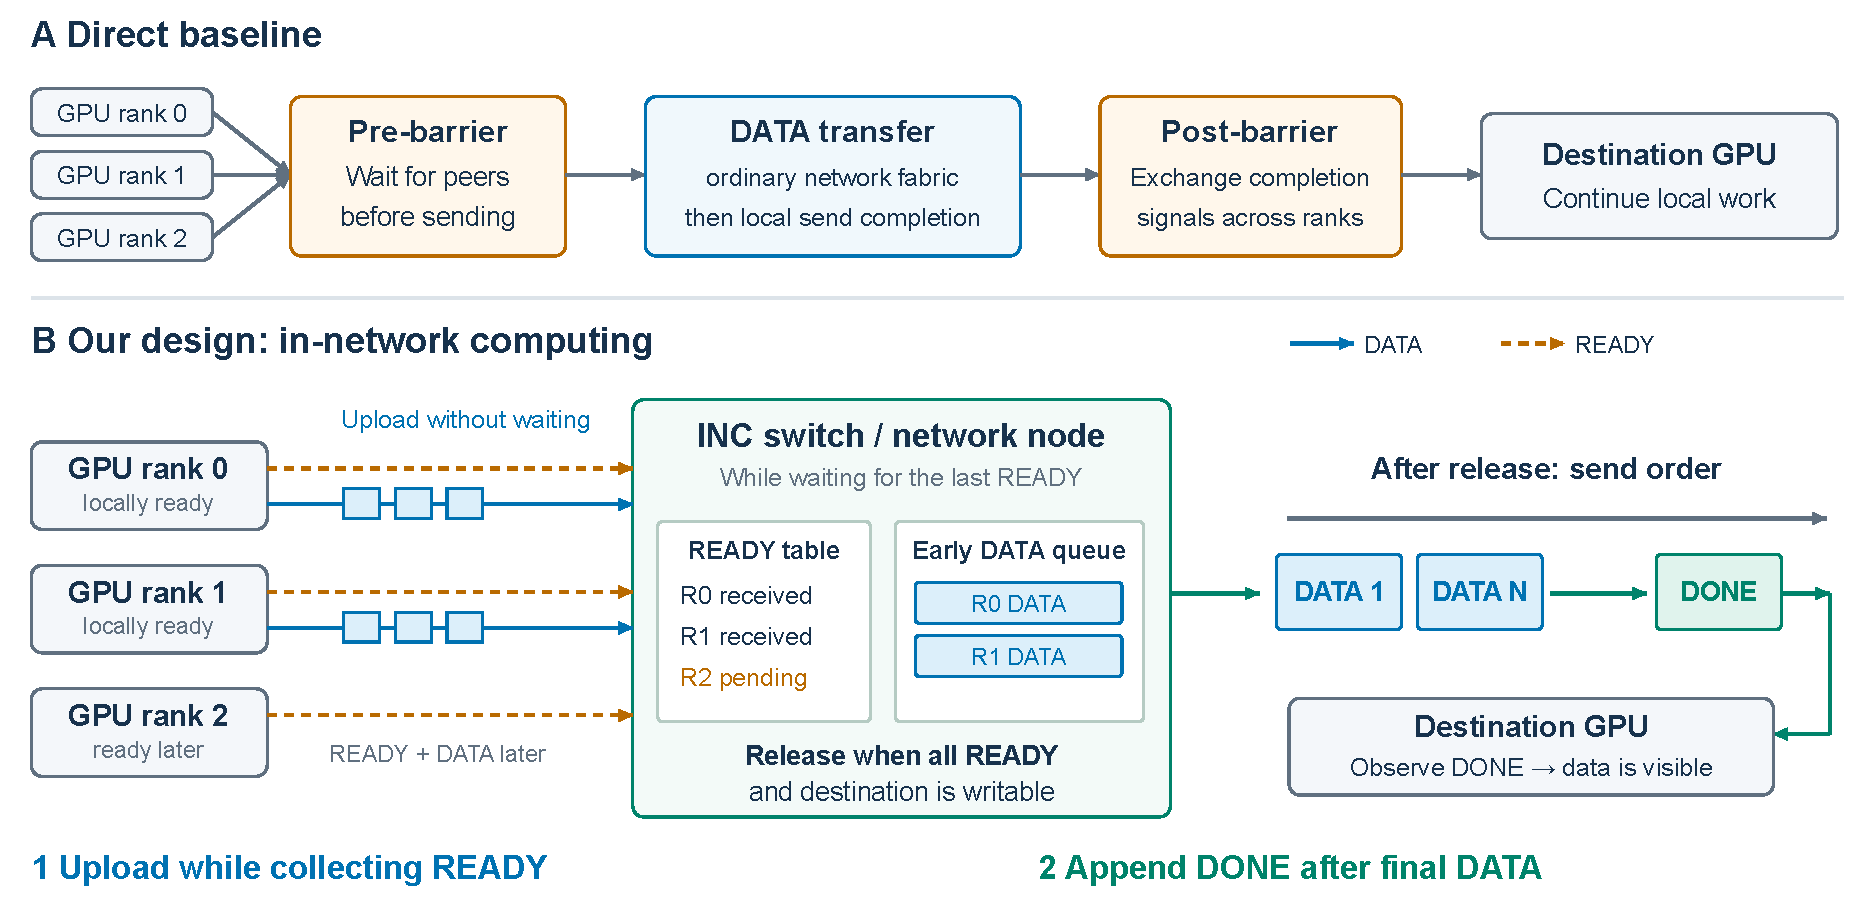
\includegraphics[width=\textwidth]{figures/inc-overview.pdf}
\caption{Two changes to Direct coordination: upload data while collecting READY, then append ordered DONE after the destination's final data. The queue shows the waiting stage; the right-hand sequence shows transmission after forwarding starts. Destination writability, data visibility, and buffer-lifetime requirements remain.}
\Description{The Direct baseline serializes pre-barrier, data transfer and sender completion, and post-barrier. With INC, ranks zero and one upload while rank two is not yet ready. The network stores READY state and early data. Once all ranks are ready, it sends data followed by DONE to the destination.}
\label{fig:design-overview}
\end{figure*}

The logical \sys{} node observes all readiness announcements and data covered by its completion decisions. For each generation it maintains (i) a participant bitmap, (ii) sealed per-destination traffic plans, (iii) output progress, (iv) destination memory descriptors, and (v) bounded staging. A generation identifies the communication instance, direction, and buffer epoch. The EP membership is known; routing determines the per-destination traffic. We assume reliable delivery with an ordering guarantee: data covered by \done{} is visible in GPU memory before \done{} is observed.

Before upload, the source obtains admission to network staging. Each destination publishes its reserved staging region, capacity, access rights, and epoch. Staging addresses must be resolvable without global receive counts, for example using a source-reserved region and a per-destination record ordinal. Each token carries its routing information and record identity, allowing INC to determine its destinations and staging positions as it arrives. Compact expert placement can be computed separately.

All traffic counted by the node must pass through its observation and completion domain. With multiple rails or nodes, progress must be partitioned and joined explicitly. Any local bypass requires a separate completion check at the consumer. The single-node measurements in Section~\ref{sec:e2e} are reference measurements; the design does not assume that an Ethernet node observes local NVLink traffic.

\subsection{Readiness Aggregation and Early Upload}
\label{sec:early-upload}
After routing and local preparation, source $s$ sends \ready{} together with a count vector: element $d$ gives its planned number of output records for destination $d$. It then uploads admitted \data{} without waiting for other ranks. INC marks a source ready only after accepting its complete vector; duplicate announcements are ignored. The node buffers early data and begins accumulating vectors as they arrive.

Once all required \ready{} messages have arrived and destination staging is writable, INC parses token routes and fans out buffered and arriving data, subject to output capacity. Vector accumulation proceeds in parallel and need not finish before fan-out starts. Thus, readiness receipt gates forwarding, while finalized counts gate completion notification. Local routing and count-vector construction remain source-side work.

The readiness dependency remains: the network cannot deliver into an unready destination. What changes is that the source-to-node transfer can proceed while readiness is being aggregated. The node's location permits this transfer to share the eventual data path. Whether the head start reduces operation latency depends on the slowest required source and the output queue, as analyzed in Section~\ref{sec:readiness-analysis}.

For Dispatch, global receive counts and final expert offsets can be computed alongside transfers into reserved staging. Count-vector entries must match the records actually emitted by fan-out, including any replication. Hardware can pipeline the integer additions with upload and forwarding; any remaining aggregation delay is included in completion latency. Multicast bandwidth savings are separate from the synchronization mechanism.

\subsection{Completion Notification}
\label{sec:completion-design}
For Dispatch generation $g$, the count vector from source $s$ contains $n_{g,s,d}$ unique output records for destination $d$. INC accumulates these vectors to obtain
\begin{equation}
 N_{g,d}=\sum_s n_{g,s,d}.
 \label{eq:count}
\end{equation}
The expected count becomes valid only after every required source has supplied its complete vector and all additions have finished. A zero entry explicitly reports no traffic; silence does not. Planned counts and output progress use the same record unit, with a fragmented record counted only when all its fragments have been submitted. Input packets, multicast replicas, and reduced outputs require their own accounting.

The node appends \done$(g,d)$ only when $N_{g,d}$ is valid and all $N_{g,d}$ records have entered the appropriate ordered delivery channel. If data finishes first, DONE waits for the final count; a destination with zero expected records is notified once its count is valid and it is ready. At the receiver, the required contract is
\begin{equation}
 \operatorname{observe}_d(\done(g,d))
 \Rightarrow
 \bigwedge_{x\in\mathcal{D}_{g,d}}\operatorname{visible}_d(x),
 \label{eq:visible}
\end{equation}
where $\mathcal{D}_{g,d}$ is the complete expected input. Output progress determines when a notification may be generated; the transport and receiver must separately establish this visibility implication.

NCCL GIN's strong-signal ordering applies to preceding PUTs to the same peer on the same context~\cite{gindocs}. A network-generated notification needs an equivalent delivery contract. Separate contexts or rails require a join, and a subsequent local forwarding hop requires its own visibility check. The distinction is about the ordering domain, not simply whether communication is within or across nodes.

Reliable delivery and duplicate suppression must precede logical progress accounting. Retransmitted fragments must not make a counter reach its target while another fragment is missing.

\done$(g,d)$ proves completion for destination $d$, rather than completion of all consumers in the EP group. A successor can use it only when destination-local completion, layout readiness, and the remaining local dependencies are sufficient. Applications that require a genuine global join retain it.

For Combine, the token owner establishes the expected contributor set during Dispatch. Contributions are identified by route slot, since several experts can occupy the same rank. Producers send weighted partials; an existing in-network reduction mechanism accumulates the expected fragments and produces the result~\cite{dysharp,switchml}. The node separately tracks input-contribution completion and reduced-output completion before notifying the owner. We attribute neither the arithmetic mechanism nor its bandwidth benefit to the synchronization design.

\subsection{Buffer Management and Progress}
\label{sec:resources}
A destination's readiness announcement commits its receive slot to the current epoch until the generation has finished using it. After observing \done{} and satisfying local requirements, Dispatch can compact the received records for expert computation; Combine can release the reduced result to its consumer. The last consumer then publishes \recycle{} and permits reuse. Emitting \done{} alone never permits overwrite.

The sender also retains its source buffer until the transport has finished reading it. Generating target notification in the network decouples the target's release from the sender's completion path; it does not remove source-lifetime tracking. Different generations therefore require separate ownership state.

Network capacity covers early arrivals, input/output imbalance after release, and any reduction accumulators. Admission must respect this capacity. When space is exhausted, unadmitted data waits at the source and continues on the same path when resources become available.

Control messages need guaranteed progress: a full data queue must not block the \ready{} messages needed to release it. Reserved control resources or an equivalent queue separation are required. PFC may provide link-level protection~\cite{pfc}, but its use does not remove the need for headroom, admission, and deadlock analysis. Capacity pressure can reduce overlap or throughput. Recovery from endpoint or network-node failure is outside the assumed reliable-delivery model.

\section{Latency Analysis}
\label{sec:model}
We model a complete Dispatch or Combine operation as READY, data transfer, and post-barrier. INC starts upload after issuing READY, overlapping data movement with the wait for peer readiness.

\subsection{Communication Latency Model}
\label{sec:delay-model}
Let $T_{\rm ready}$ be the pre-barrier duration, $T_{\rm data}$ the data-transfer phase, and $T_{\rm post}$ the post-barrier and subsequent local epilogue. The data phase includes the sender-side work needed to enter the post-barrier. The baseline executes these stages in sequence:
\begin{equation}
 T_{\rm base}=T_{\rm ready}+T_{\rm data}+T_{\rm post}.
 \label{eq:base}
\end{equation}

Following Swift's separation of processing and network delay~\cite{swift}, consider a reference with simultaneous rank readiness and comparable communication paths:
\begin{equation}
 T_{\rm ready}=T_{\rm local}+T_{\rm signal}.
 \label{eq:ready}
\end{equation}
Here $T_{\rm local}$ includes preparing, issuing, and checking readiness signals. $T_{\rm signal}$ is the network time for the required signal exchange. With concurrent announcements and symmetric paths, this exchange requires one one-way traversal, approximately half a network RTT.

\subsection{Latency Reduction from Early Upload}
\label{sec:readiness-analysis}
In the baseline, ranks finish the entire READY stage before sending DATA. With INC, each rank issues READY and starts uploading. READY and DATA travel toward the network node together; INC holds any early data until the required signals have arrived and destination buffers are writable. \autoref{fig:timing} illustrates this change in timing.

% Schematic timing of endpoint coordination and the proposed \sys{} path.
% Coordinates are schematic, not measurements. Dashed = control; solid = \data{}.
\begin{figure*}[t]
\centering
\begin{tikzpicture}[x=1cm,y=-1cm,font=\footnotesize]
\path[use as bounding box] (0,0) rectangle (17.5,9.3);
\begin{scope}[shift={(0,4.75)}]
\node[paneltitle] at (.1,.15) {(c) Aligned ranks: endpoint exchanges};
\node at (1.1,.65) {Rank 0}; \node at (5.7,.65) {Rank 1};
\draw[lifeline] (1.1,.9)--(1.1,4.2); \draw[lifeline] (5.7,.9)--(5.7,4.2);
\draw[ctrlarrow] (1.1,1.05)--(5.7,1.65);
\draw[ctrlarrow] (5.7,1.05)--(1.1,1.65);
\node[smalllabel] at (3.4,1.08) {\ready{} all-to-all};
\foreach \y in {1.8,2.04,2.28,2.95} {
\draw[dataarrow] (1.1,\y)--(5.7,{\y+.6});
\draw[dataarrow] (5.7,\y)--(1.1,{\y+.6});}
\draw[ctrlarrow] (1.1,3.62)--(5.7,4.17);
\draw[ctrlarrow] (5.7,3.62)--(1.1,4.17);
\node[smalllabel] at (3.4,3.94) {completion exchange};
\draw[<->] (6.1,1.05)--(6.1,1.65) node[midway,right,align=left] {pre\,$\simeq L$};
\draw[<->] (6.1,3.62)--(6.1,4.17) node[midway,right,align=left] {post\,$\simeq L$};
\end{scope}
\begin{scope}[shift={(8.8,4.75)}]
\node[paneltitle] at (.1,.15) {(d) Aligned ranks: \sys{} overlap};
\node at (.8,.65) {Rank 0}; \node at (3.6,.65) {\sys{}}; \node at (6.4,.65) {Rank 1};
\foreach \x in {.8,3.6,6.4} \draw[lifeline] (\x,.9)--(\x,4.2);
\draw[ctrlarrow] (.8,1.05)--(3.6,1.35); \draw[ctrlarrow] (6.4,1.05)--(3.6,1.35);
\fill[incgreen] (3.6,1.35) circle (.045);
\node[smalllabel,anchor=west] at (3.75,1.08) {all \ready{}};
\foreach \y in {1.2,1.44,1.68,2.35} {
\draw[dataarrow] (.8,\y)--(6.4,{\y+.6});
\draw[dataarrow] (6.4,\y)--(.8,{\y+.6});}
\draw[ctrlarrow] (3.6,2.72)--(6.4,3.02);
\draw[ctrlarrow] (3.6,2.72)--(.8,3.02);
\node[smalllabel,align=center] at (3.6,3.44) {\done{} follows final \data{}\\on each ordered output};
\node[anchor=west] at (.4,4.02) {No sender release wait; no new endpoint exchange.};
\end{scope}
\begin{scope}[shift={(0,0)}]
\node[paneltitle] at (.1,.15) {(a) Unequal ranks: endpoint exchanges};
\node at (1.1,.65) {Rank 0}; \node at (5.7,.65) {Rank 1};
\draw[lifeline] (1.1,.9)--(1.1,4.3); \draw[lifeline] (5.7,.9)--(5.7,4.3);
\draw[ctrlarrow] (1.1,1.0)--(5.7,1.6); \draw[ctrlarrow] (5.7,1.55)--(1.1,2.15);
\node[smalllabel] at (3.4,1.02) {Rank 1 ready later};
\foreach \y in {2.2,2.43,2.66,3.03} \draw[dataarrow] (1.1,\y)--(5.7,{\y+.6});
\foreach \y in {1.65,1.88,2.11,2.48} \draw[dataarrow] (5.7,\y)--(1.1,{\y+.6});
\draw[ctrlarrow] (1.1,3.2)--(5.7,3.8);
\draw[ctrlarrow] (5.7,3.72)--(1.1,4.32);
\node[smalllabel,align=center] at (3.4,4.15) {Readiness and completion\\still traverse between endpoints};
\end{scope}
\begin{scope}[shift={(8.8,0)}]
\node[paneltitle] at (.1,.15) {(b) Unequal ranks: bounded staging};
\node at (.8,.65) {Rank 0}; \node at (3.6,.65) {\sys{}}; \node at (6.4,.65) {Rank 1};
\foreach \x in {.8,3.6,6.4} \draw[lifeline] (\x,.9)--(\x,4.3);
\fill[pattern=north east lines,pattern color=black!35] (3.43,1.43) rectangle (3.77,1.87);
\draw[ctrlarrow] (.8,1.0)--(3.6,1.3);
\draw[ctrlarrow] (6.4,1.55)--(3.6,1.85);
\draw[dataarrow] (.8,1.13)--(3.6,1.43);
\draw[dataarrow] (.8,1.36)--(3.6,1.66);
\draw[dataarrow] (.8,1.59)--(3.6,1.89);
\draw[dataarrow] (3.6,1.9)--(6.4,2.2);
\draw[dataarrow] (3.6,2.13)--(6.4,2.43);
\draw[dataarrow] (3.6,2.36)--(6.4,2.66);
\draw[dataarrow] (.8,2.18)--(3.6,2.48)--(6.4,2.95);
\foreach \y in {1.68,1.91,2.14,2.51} \draw[dataarrow] (6.4,\y)--(.8,{\y+.6});
\draw[ctrlarrow] (3.6,2.72)--(6.4,3.02);
\draw[ctrlarrow] (3.6,2.88)--(.8,3.18);
\node[smalllabel,anchor=east] at (3.2,1.68) {buffer};
\node[smalllabel,align=center] at (3.6,3.6) {Wait for \ready{} at the \sys{} node;\\preserve output service and ordering};
\node[anchor=west] at (.4,4.18) {Skew coverage is not an additional fixed saving.};
\end{scope}
\end{tikzpicture}
\caption{Idealized projection of the two-boundary design, not a measured Direct trace. Solid arrows carry \data{}; dashed arrows carry control. The left-hand reference assumes an exposed tail-signal interval of approximately $L$ after data arrival; actual Direct timing follows Equation~\eqref{eq:tailgain}. \sys{} overlaps readiness with upload and appends ordered \done{} at each destination's tail. Early data is buffered under skew. Required local completion and buffer ownership are retained.}
\Description{Four timing panels compare endpoint and network coordination. The top pair shows unequal readiness and buffering; the lower pair shows aligned readiness as an ideal reference. Solid arrows are data and dashed arrows are control.}
\label{fig:timing}
\end{figure*}


To isolate the benefit of overlap, we retain the same local processing cost, data-transfer duration, and post-barrier work in the reference model. When early upload covers the signal-transfer interval, the INC latency is
\begin{equation}
 T_{\rm INC}\approx T_{\rm local}+T_{\rm data}+T_{\rm post}+T_{\rm extra}.
 \label{eq:inc}
\end{equation}
$T_{\rm extra}$ is the additional critical-path delay introduced by INC processing, buffering, and forwarding waits. The ordinary source-to-destination DATA transfer is already included in $T_{\rm data}$; local processing remains accounted for in $T_{\rm local}$.

The reference difference is therefore
\begin{equation}
 \Delta T\approx T_{\rm signal}-T_{\rm extra}.
 \label{eq:gain}
\end{equation}
Early upload thus hides approximately half a network RTT in this reference case, less the added INC delay. The saving comes from overlapping signal transmission with data movement, while the post-barrier remains unchanged.

\subsection{Overlap with Unequal Readiness}
\label{sec:skew}
In practice, differences in computation and scheduling often make ranks ready at different times. \autoref{fig:timing}(C--D) shows how the overlap works in this case: early ranks upload while later ranks prepare, and INC buffers the data. When the last required READY arrives, INC can start forwarding these tokens instead of waiting for the early ranks to receive peer signals and then begin uploading. The mechanism therefore does not require synchronized arrivals.

With sufficient staging and forwarding capacity, this upload head start is preserved under readiness skew and shortens the operation when it advances critical-path data delivery. Output queuing and PFC pauses contribute to $T_{\rm extra}$. The gain depends on the last rank to finish and the available overlap, rather than a fixed fraction of RTT for every arrival pattern.

\section{Evaluation}
\label{sec:evidence}
We characterize pre-barrier costs in Direct microbenchmarks and their contribution to MoE inference.

\subsection{Experimental Setup and Methodology}
\label{sec:setup}
Each node has eight H200 GPUs connected by NVSwitch and eight 400\,GbE RoCE interfaces. Cross-node runs use GIN's GDAKI backend, traffic class 162, PyTorch 2.13, CUDA 13, NCCL 2.31.2, and DeepEP V2 based on commit \texttt{01dc3aaa}~\cite{deepepcode}. Direct is selected with Hybrid disabled; available local communication within Direct is retained.

Microbenchmarks fix $H=7168$, $\topk=8$, 256 experts, BF16, and balanced uniform routing. $T$ denotes tokens per rank. Each point has three independent process runs with 200 active iterations per run. Error bars show the standard deviation across run means.

For each iteration, we select the rank with the shortest pre-barrier interval and divide that duration by the same rank's trace-on operator time. We average these ratios within each run and then across runs. This statistic reduces the effect of rank arrival skew, while retaining any waiting experienced by the selected rank. Phase shares use paired trace-on measurements; trace-off operator timings are kept separately.

The EP8 share sweep covers $T=8,32,64,128$. The EP-size comparison uses the original measurements at $T=8,32,96,128$, supplemented by the later EP8 $T=64$ batch. Configuration and per-run values accompany the data.

\subsection{Pre-Barrier Cost}
\label{sec:entry-eval}
Figure~\ref{fig:entry-cost} reports pre-barrier duration and operator share at EP8. Dispatch and Combine remain near 15\us{} across the measured token counts. Their shares fall from 20.57\% and 19.84\% at $T=8$ to 4.88\% and 5.05\% at $T=128$. Small batches therefore expose a larger fraction of the operation to readiness coordination.

% Frozen values: data/h200/numbers/paired_control_share.json.
\begin{figure*}[t]
\centering
\begin{minipage}{0.49\textwidth}
\centering
\begin{tikzpicture}
\begin{axis}[width=\linewidth,height=5.0cm,
 title={(a) Entry duration},xlabel={Tokens per rank},ylabel={Duration (\(\mu\mathrm{s}\))},
 xmode=log,log basis x=2,xtick={8,32,64,128},xticklabels={8,32,64,128},
 xmin=6,xmax=170,ymin=0,ymax=18,
 grid=major,grid style={black!10},axis lines=left,
 tick label style={font=\footnotesize},label style={font=\footnotesize},
 title style={font=\small},legend style={font=\footnotesize,at={(.97,.12)},anchor=south east,draw=none}]
\addplot+[datablue,mark=*,solid,error bars/.cd,y dir=both,y explicit]
 coordinates {(8,15.09) +- (0,0.06) (32,15.35) +- (0,0.46) (64,14.90) +- (0,0.10) (128,15.05) +- (0,0.21)};
\addlegendentry{Dispatch}
\addplot+[controlorange,mark=square*,dashed,error bars/.cd,y dir=both,y explicit]
 coordinates {(8,15.15) +- (0,0.03) (32,15.04) +- (0,0.22) (64,14.82) +- (0,0.13) (128,14.95) +- (0,0.23)};
\addlegendentry{Combine}
\end{axis}
\end{tikzpicture}
\end{minipage}
\hfill
\begin{minipage}{0.49\textwidth}
\centering
\begin{tikzpicture}
\begin{axis}[width=\linewidth,height=5.0cm,
 title={(b) Share of operator},xlabel={Tokens per rank},ylabel={Entry share (\%)},
 xmode=log,log basis x=2,xtick={8,32,64,128},xticklabels={8,32,64,128},
 xmin=6,xmax=170,ymin=0,ymax=24,
 grid=major,grid style={black!10},axis lines=left,
 tick label style={font=\footnotesize},label style={font=\footnotesize},
 title style={font=\small},legend style={font=\footnotesize,at={(.97,.97)},anchor=north east,draw=none}]
\addplot+[datablue,mark=*,solid,error bars/.cd,y dir=both,y explicit]
 coordinates {(8,20.57) +- (0,0.06) (32,12.25) +- (0,0.17) (64,8.29) +- (0,0.51) (128,4.88) +- (0,0.04)};
\addlegendentry{Dispatch}
\addplot+[controlorange,mark=square*,dashed,error bars/.cd,y dir=both,y explicit]
 coordinates {(8,19.84) +- (0,0.13) (32,12.26) +- (0,0.26) (64,8.20) +- (0,0.16) (128,5.05) +- (0,0.19)};
\addlegendentry{Combine}
\end{axis}
\end{tikzpicture}
\end{minipage}
\caption{H200 cross-node EP8 Direct. Entry duration stays close to 15\us{} while its operator share decreases. Both use the selected rank's trace-on measurements; error bars are standard deviations across three run means. Lines connect measured points.}
\label{fig:entry-cost}
\Description{Two panels show entry synchronization versus tokens per rank. Duration stays near fifteen microseconds for Dispatch and Combine, while operator share declines from about twenty percent to about five percent. Error bars describe three process runs.}
\end{figure*}


\subsection{Dependence on EP Size}
\label{sec:scale-eval}
Table~\ref{tab:entry-constants} summarizes pre-barrier duration with a separate constant for EP4, EP8, and EP16. All listed token counts participate in the estimate. The largest deviation of a per-token-count mean from its configuration's constant is 0.16\us{}, supporting a nearly constant cost over the measured batch range.

\begin{table}[t]
\centering
\small
\setlength{\tabcolsep}{3pt}
\begin{tabular}{@{}llrrr@{}}
\toprule
EP & Fitted $T$ & Dispatch & Combine & Max. dev.\\
\midrule
4 & 8/32/96/128 & 11.65 & 11.54 & 0.06\\
8 & 8/32/64/96/128 & 14.96 & 14.94 & 0.16\\
16 & 8/32/96/128 & 18.36 & 18.28 & 0.09\\
\bottomrule
\end{tabular}
\caption{Pre-barrier constants and maximum deviation of per-$T$ run means, in \(\mu\mathrm{s}\). Each $T$ has three process runs. EP8 includes a later $T=64$ batch with different instrumentation.}
\label{tab:entry-constants}
\end{table}

The fitted duration rises from approximately 11.6\us{} at EP4 to 18.3\us{} at EP16. These configurations change GPUs per node, traffic destinations, and network concurrency together, so the observed variation reflects their combined effect.

\subsection{Pre-Barriers in MoE Inference}
\label{sec:e2e}
We measure Qwen3-30B-A3B in BF16 with vLLM 0.27 and DeepEP V2 Direct. The model has $H=2048$, 128 experts, and $\topk=8$. Runs use actual routing, TP=1, EP8, and requests with 128 input and 128 output tokens. We compare one node with eight ranks to two nodes with four ranks each, at concurrency 64 and 128.

The serving build includes tracing and an expert-padding correctness fix. Each sampled active rank has 48 Dispatch and 48 Combine trace entries per decode step. We sum its pre-barrier intervals, divide by that rank's GPU-step time, and average over ranks and three client windows on the same server instance.

% Source: outline_shares.json, e2e[].pre_share_percent only.
\begin{figure}[t]
\centering
\begin{tikzpicture}
\begin{axis}[width=\columnwidth,height=5.4cm,
 ybar,bar width=12pt,symbolic x coords={64,128},xtick=data,
 xlabel={Request concurrency},ylabel={Pre-barrier share of GPU step (\%)},
 enlarge x limits=0.45,ymin=0,ymax=22,
 grid=major,grid style={black!10},
 tick label style={font=\footnotesize},label style={font=\footnotesize},
 legend style={font=\footnotesize,at={(.5,.98)},anchor=north,legend columns=2,draw=none}]
\addplot+[fill=datablue!45,draw=datablue,error bars/.cd,y dir=both,y explicit]
 coordinates {(64,9.33) +- (0,0.12) (128,7.94) +- (0,0.15)};
\addlegendentry{1 node}
\addplot+[pattern=north east lines,pattern color=controlorange,draw=controlorange,error bars/.cd,y dir=both,y explicit]
 coordinates {(64,16.72) +- (0,0.10) (128,15.19) +- (0,0.05)};
\addlegendentry{2 nodes}
\end{axis}
\end{tikzpicture}
\caption{Qwen3-30B-A3B decode at fixed EP8. Pre-barrier intervals for Dispatch and Combine are paired with the same rank's GPU step. Error bars describe three client windows, not server restarts.}
\label{fig:inference-share}
\Description{Grouped bars compare one-node and two-node EP8 decode at request concurrency sixty-four and one hundred twenty-eight. Single-node pre-barrier shares are around eight to nine percent, and cross-node shares around fifteen to seventeen percent.}
\end{figure}


At concurrency 64, the pre-barrier share is 9.33\% within one node and 16.72\% across two nodes. At concurrency 128, the corresponding values are 7.94\% and 15.19\%. Thus, readiness coordination remains visible in the full decode step with real routing and model computation.

These percentages describe sampled GPU steps. Unlike the microbenchmark statistic, they average over ranks rather than selecting the shortest interval. Together, the two experiments show both the operator-level cost and its place in inference.

\section{Related Work}
\label{sec:related}

\subsection{EP Communication}
DeepEP~\cite{deepep} and NCCL EP~\cite{ncclep} provide GPU-initiated communication paths for expert parallelism. Their metadata exchanges, preallocated buffers, and synchronization schedules determine when data can be sent. \sys{} uses network staging to begin upload while peer readiness is still being collected.

SwiftEP~\cite{swiftep} optimizes buffer movement and GPU work, while COMET~\cite{comet} overlaps communication with computation. Perseus~\cite{perseus} reorganizes PUT, fence, and signal processing in the transfer pipeline. UBEP~\cite{ubep} uses point-to-point signals and Data-as-Flag to reduce stage synchronization in scale-up EP. These approaches improve data movement or its coordination; early upload complements them when a readiness dependency precedes transmission.

\subsection{In-Network Computation}
SHARP~\cite{sharp} and SwitchML~\cite{switchml} use network computation for collective reduction. DySHARP~\cite{dysharp} combines dynamic addressing, multicast, and reduction for MoE, while MultiWrite~\cite{multiwrite} uses multicast writes to reduce repeated upstream transfers. These systems demonstrate network processing and state management for distributed workloads. \sys{} applies temporary state and buffering to overlap pre-barrier coordination with upload.

\subsection{Synchronization and Delay Analysis}
EPIC~\cite{epic} provides protocol and resource abstractions for Ethernet in-network computing. GPU-initiated networking~\cite{gin} provides endpoint communication primitives. \sys{} combines these capabilities with readiness checks, symmetric receive buffers, and flow control.

Swift~\cite{swift} separates processing and network contributions to delay. We apply that distinction to the execution order of an EP operation. FabricPerf~\cite{fabricperf} further motivates explicit timing boundaries; our pre-barrier measurements pair each interval with the corresponding operator or GPU step.

\section{Conclusion}
Cross-node DeepEP V2 Direct places coordination before payload injection and after sender-side completion work. H200 measurements show that entry synchronization remains near 15\us{} at EP8 across the measured small-batch points and occupies 15.2--16.7\% of the sampled cross-node MoE decode step. \sys{} proposes to overlap readiness aggregation with upload and to generate ordered completion notification at the network output. Its benefit depends on data visibility, buffer ownership, bounded staging, and the delay exposed on the consumer's critical path. The protocol and model describe this opportunity; evaluating its net performance requires an implementation.

\label{end:body}

% Keep normal two-column pagination rather than forcing the bibliography to balance.
\bibliographystyle{ACM-Reference-Format}
\bibliography{references}

\end{document}
